% !TeX program = xelatex
% 第二章 2.1、2.2。接在 \chapter{研究系統介紹} 之後。
% 規格區分官方硬體數值與本研究模擬設定，不推定實機感測器型號。

% ==================================================
% 2.1 移動機械臂平台
% ==================================================
\section{移動機械臂平台}
\label{sec:mobile_manipulator_platform}

本研究平台由四輪全向底盤、六軸 Lite 6 手臂、平行夾爪、二維雷射掃描與手腕 RGB-D 相機組成。底盤提供平面內兩方向平移與旋轉自由度，手臂提供末端位置及姿態調整，兩者共同形成九自由度的運動描述。平台幾何及命令設定整理於\cref{tab:platform_specifications}；Lite 6 硬體規格依官方資料列示\cite{ufactorylite6specs}，輪系與模擬感測參數依本研究模型及執行設定列示。

\begin{table}[htbp]
    \centering
    \caption{移動機械臂平台與模擬感測設定}
    \label{tab:platform_specifications}
    \begingroup
    \small
    \renewcommand{\arraystretch}{1.25}
    \begin{tabular}{|p{0.18\textwidth}|p{0.50\textwidth}|p{0.22\textwidth}|}
        \hline
        項目 & 規格或設定 & 資料性質 \\
        \hline
        全向輪配置 & 四輪十字配置，輪心位於底盤前、左、後、右側 & 本研究模型 \\
        \hline
        輪徑與輪距 & 輪徑 $0.10$ m；車心至輪心距離 $L=0.245$ m & URDF 與輪系參數 \\
        \hline
        底盤尺寸與輪速 & 底盤外半徑 $0.30$ m；單輪角速度上限 $5.55$ rad/s & 模型與控制限制 \\
        \hline
        Lite 6 手臂 & 六軸；工作半徑 $440$ mm；額定負載 $600$ g & 官方硬體規格 \\
        \hline
        平行夾爪 & Lite Gripper；官方開合行程 $16$ mm、夾持力 $5$ N；模擬開度與接觸力依實驗另列 & 官方規格／模擬設定分列 \\
        \hline
        二維雷射掃描 & $360$ 束、全周掃描、$10$ Hz；模擬量測範圍 $0.12$--$10$ m & 模擬參數，非實機型號規格 \\
        \hline
        手腕 RGB-D 相機 & D435 外形模型；$640\times480$、水平視角 $69^{\circ}$；第 97 趟送入偵測之頻率 $5$ Hz & 模型及該趟執行設定 \\
        \hline
    \end{tabular}
    \endgroup
\end{table}
% 幾何：evaluation/models/omni_bot_wholebody_expanded.urdf。
% 雷射：src/my_omnibot_description/urdf/lidar.xacro、evaluation/isaac_m8_house_d2.py。
% 第 97 趟相機與增益：evaluation/runs/m8house_d2_unified_97/result.json readback。

% ==================================================
% 2.1.1 全向移動底盤
% ==================================================
\subsection{全向移動底盤}
\label{subsec:omnidirectional_mobile_base}

四個全向輪沿底盤中心以 $90^{\circ}$ 間隔配置，各輪沿切向提供驅動速度，輪緣滾子則允許側向運動。底盤控制輸入為本體座標中的 $v_x$、$v_y$ 與偏航角速度 $\omega$。平移與旋轉同時發生時，各輪的速度需求具有耦合關係，控制器及執行端因此同時考量輪速及輪速變化限制；其數學關係於第三章說明。

% ==================================================
% 2.1.2 六軸機械臂與夾爪
% ==================================================
\subsection{六軸機械臂與夾爪}
\label{subsec:lite6_arm_gripper}

Lite 6 安裝於底盤中心前方 $0.11$ m，其基座相對底盤 \texttt{base\_link} 的平移為 $(0.11,0,0.28)$ m。底盤平面基準座標 $\mathcal F_B$ 對應 \texttt{base\_footprint}，而 \texttt{base\_link} 位於其上方 $0.05$ m，因此手臂基座相對平面基準的平移為 $(0.11,0,0.33)$ m，與第三章的固定變換定義一致。夾爪工具中心點（Tool Center Point, TCP）作為操作追蹤之末端座標；手腕相機透過固定外參連結至手臂末端。整機座標配置如\cref{fig:robot_coordinate_frames}所示，以 $x_B$ 指向前方、$y_B$ 指向左方、$z_B$ 指向上方。手臂基座、TCP、相機及光達之座標轉換由模型中的固定與轉動關節共同決定。

\begin{figure}[htbp]
    \centering
    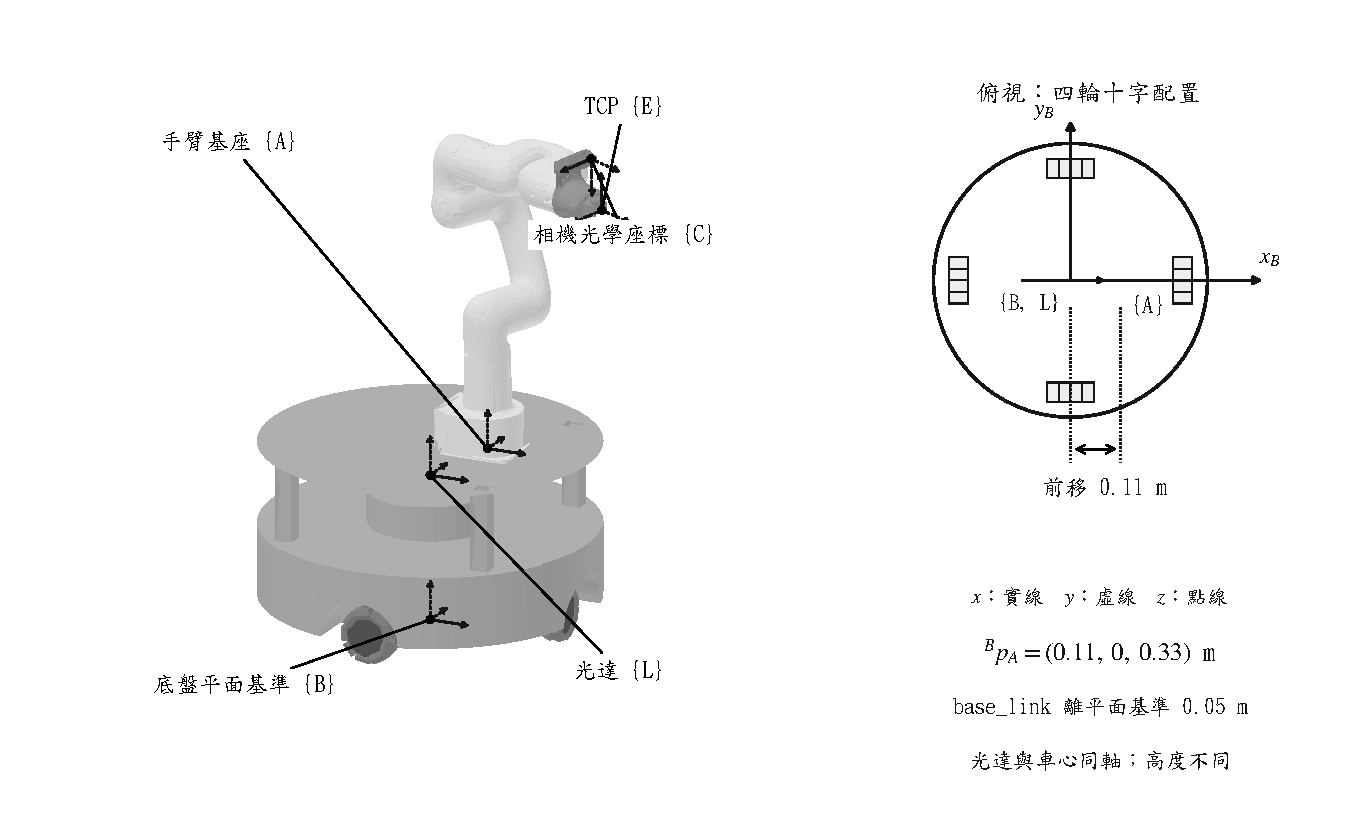
\includegraphics[width=0.98\textwidth]{figsrc/ch02/robot_coordinate_frames.pdf}
    \caption{移動機械臂之座標配置與四輪十字排列；手臂基座相對底盤中心前移 $0.11$ m}
    \label{fig:robot_coordinate_frames}
\end{figure}

% ==================================================
% 2.2 感測設備與命令介面
% ==================================================
\section{感測設備與命令介面}
\label{sec:sensors_command_interfaces}

% ==================================================
% 2.2.1 雷射掃描與深度相機
% ==================================================
\subsection{雷射掃描與深度相機}
\label{subsec:lidar_depth_camera}

二維雷射資料提供導航代價地圖、障礙運動估測及近距離防護所需之回波。光達與底盤中心於水平面上重合，在模型中的離地高度為 $0.2652$ m。手腕 RGB-D 相機提供操作物件的彩色影像及深度，經分割及幾何估測後生成操作目標。影像與深度以擷取時間及相機座標識別，使用該時刻的底盤及關節狀態完成座標轉換。若配置另啟用機身相機，則保留來源識別與各自外參，不與未啟用該相機的批次混用。

% ==================================================
% 2.2.2 底盤里程與關節狀態回授
% ==================================================
\subsection{底盤里程與關節狀態回授}
\label{subsec:odometry_joint_feedback}

底盤位姿與里程資料用於導航定位及幾何追蹤誤差計算；手臂回授包含六軸關節位置。控制端另保存各關節位置設定點，以區分要求位置與實際位置。實際放行速度、設定點、來源時間與序號共同提供予後續預測。各模擬批次使用的位姿來源與定位配置於第四章分別揭露。

模擬器提供的手指位置與接觸力用於判定該模擬模型下的抓持證據。Lite 6 實機夾爪之開合命令與可取得訊號須依實際介面確認；模擬手指接觸量不視為實機已具備的原生回授。採用固定連接承載物件時，亦於實驗中揭露理想抓持假設。

% ==================================================
% 2.2.3 底盤速度與手臂位置命令介面
% ==================================================
\subsection{底盤速度與手臂位置命令介面}
\label{subsec:base_arm_command_interfaces}

命令處理關係如\cref{fig:command_execution_chains}所示。底盤速度依序通過命令平滑、原始雷射防護及輪級限制，最終放行值才是執行端實際採用的速度。控制器使用此值更新後續預測及命令差分，使防護修正能回到閉迴路。

手臂最佳化輸出為關節位置設定點的變化率，經離散積分形成位置設定點，再由模擬中的關節 PD 追蹤。第 97 趟六軸增益讀回皆為 $k_p=600$、$k_d=60$，其概念形式為 $\tau_a=k_p(s_a-q_a)-k_d\dot q_a$。這些數值為 Isaac 致動設定，實際運動仍受物理求解、限幅及負載影響；第三章以等效設定點追蹤模型建立預測，並分別處理命令延遲與模型偏置。

\begin{figure}[htbp]
    \centering
    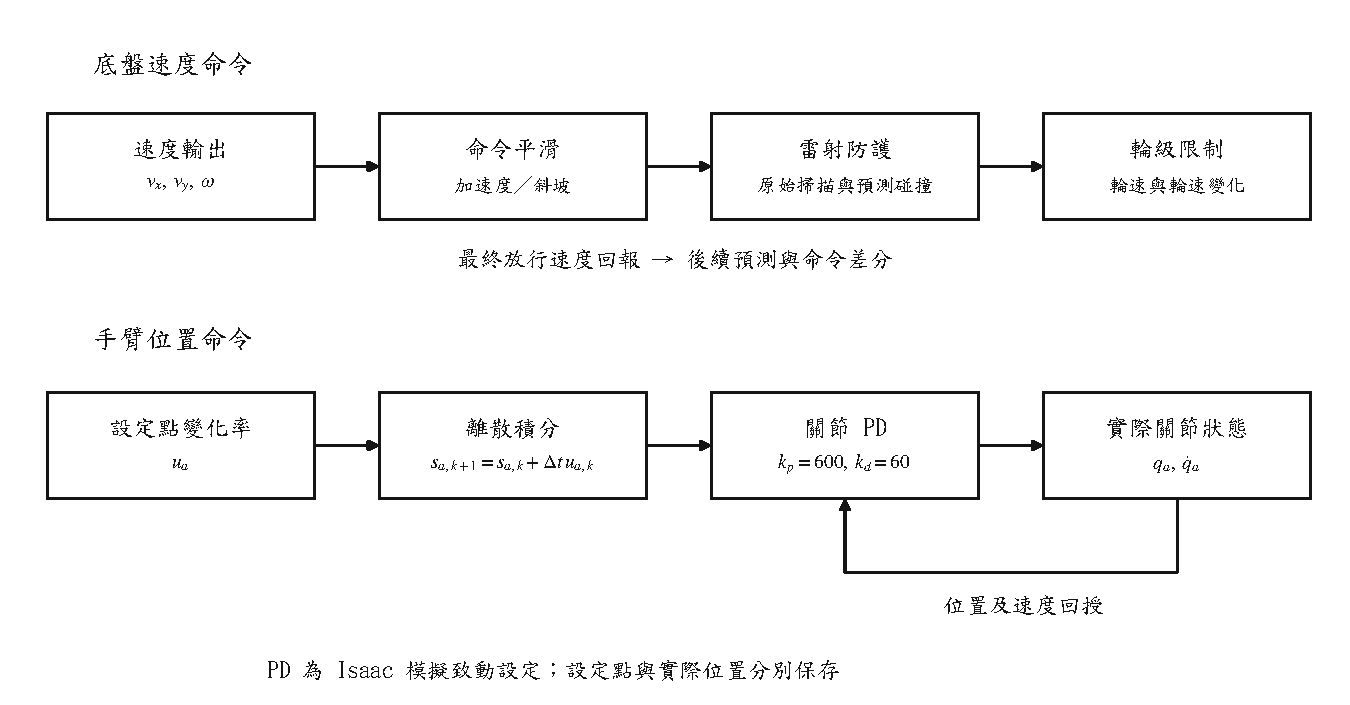
\includegraphics[width=0.98\textwidth]{figsrc/ch02/command_execution_chains.pdf}
    \caption{底盤速度與手臂位置設定點之命令執行鏈；PD 增益為 Isaac 模擬設定}
    \label{fig:command_execution_chains}
\end{figure}
